\subsection{Structure}

\subsubsection{Block Definition Diagram}
The system consist of three parts, a random generator, an user interface and the particle swarm logic. on Figure \ref{fig:bdd} the block definition diagram can be seen with these three parts, as part of the overall Particle Swarm Optimization System.

\begin{figure}[!h]
	\centering
	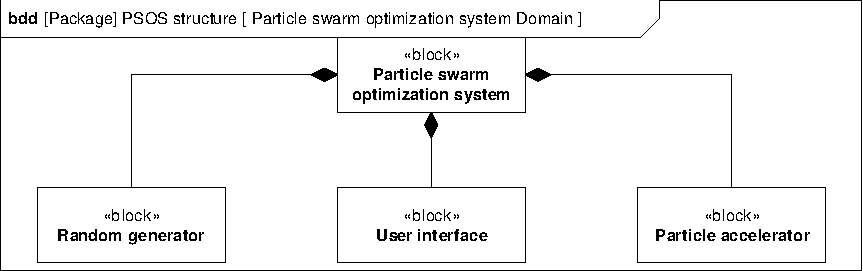
\includegraphics[width=0.8\linewidth]{diagram/bdd_particle_swarm_optimization_system.pdf}
	\caption{Block Definition Diagram}
	\label{fig:bdd}
\end{figure}

\textbf{Random Generator:}\\
The Random Generator block is needed, to generate random seeds for use in the particle swarm algorithm.\\

\textbf{User Interface:}\\
The User Interface block needs core functionality to communicate with the system. It needs to be able to take inputs regarding the particle swarm algorithms variables and create a graphical representation of the results to the user, after a successful particle swarm analysis.\\

\textbf{Particle Accelerator:}\\
The Particle Accelerator block has the functionality to perform the particle swarm optimization algorithm. Variables for the algorithm, given by the user, are communicated via the User Interface block. The random seed for the algorithm is given by the Random Generator block.

\subsubsection{Internal Block Diagram}


\begin{figure}[!h]
	\centering
	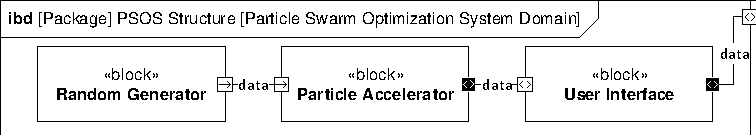
\includegraphics[width=0.8\linewidth]{diagram/ibd_particle_swarm_optimization_system.pdf}
	\caption{Internal Block Diagram}
	\label{fig:ibd}
\end{figure}
